\begin{figure}[htbp]
    \captionsetup[subfigure]{justification=centering}
    \centering
    \begin{subfigure}[b]{0.3\textwidth}
        \centering
        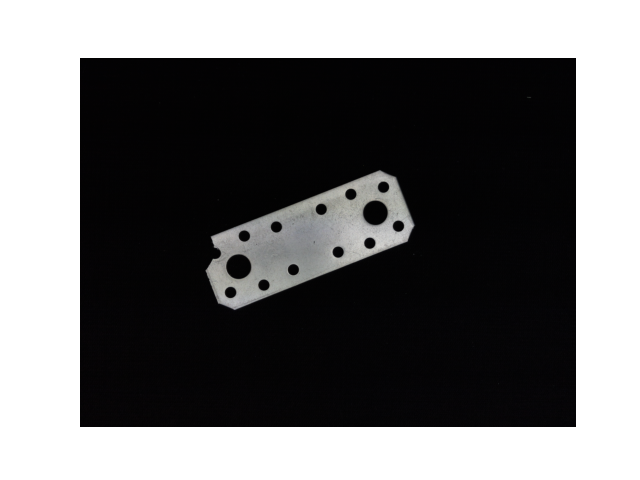
\includegraphics[width=\textwidth]{figures/pca_results/cut_corner.png}
        \caption*{Original Image}

    \end{subfigure}
    \begin{subfigure}[b]{0.3\textwidth}
        \centering
        
\includegraphics[width=\textwidth]{figures/pca_results/cut_corner_mask.png}
        \caption*{Mask}

    \end{subfigure}
    \begin{subfigure}[b]{0.3\textwidth}
        \centering
        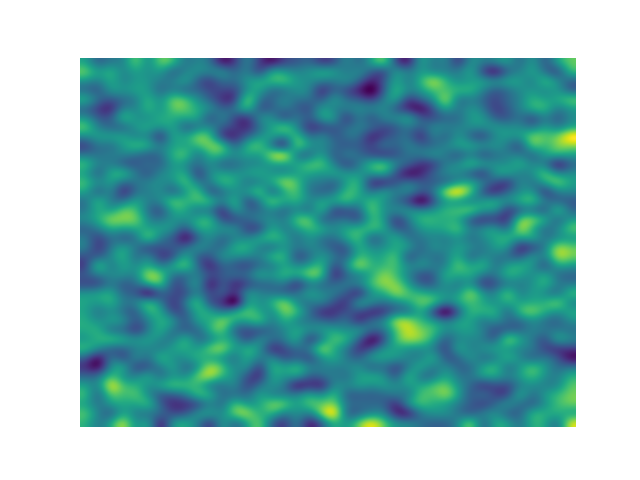
\includegraphics[width=\textwidth]{figures/pca_results/pca_res.png}
        \caption*{Discriminator Predictions}

    \end{subfigure}
    \caption{Results of using the Independent Transformation Block \cite{EnsembleHeller2023} for the ensemble process for the flat connector class. 
             These results are also produced when just applying PCA to a single ensemble member and training with it.}
    \label{fig:pca_res}
\end{figure}